\chapter{User Study Questionnaires and Interview Protocols}
\label{appendix:questionnaires}

This appendix contains the complete questionnaires and interview protocols used in the user study. The materials are organized into two main sections: standardized questionnaires and interview protocols.

\section{Standardized Questionnaires}

\subsection{Demographic Questionnaire}
\label{appendix:demographic-questionnaire}

The demographic questionnaire collected background information about participants and their relevant experience.

\begin{enumerate}
    \item Please select your gender:
    \begin{itemize}
        \item Male
        \item Female
        \item Non-binary
        \item Prefer not to say
        \item Enter yourself
    \end{itemize}
    
    \item Please state your age: \underline{\hspace{3cm}}
    
    \item What is your native language? \underline{\hspace{5cm}}
    
    \item Please select your current employment status:
    \begin{itemize}
        \item Student (incl. PhD)
        \item Staff
        \item Enter yourself
    \end{itemize}
    
    \item How would you rate your experience with Augmented Reality (AR) and Virtual Reality (VR) applications?
    \begin{itemize}
        \item No experience
        \item Limited experience
        \item Moderate experience
        \item Extensive experience
    \end{itemize}
    
    \item If applicable, please specify the AR/VR devices or applications you have used: \underline{\hspace{8cm}}
    
    \item What types of AR/VR applications have you interacted with? (Select all that apply)
    \begin{itemize}
        \item Gaming
        \item Training/Simulation
        \item Industrial Prototyping
        \item Collaboration
        \item Other
    \end{itemize}
    
    \item How would you rate your experience with assembly or prototyping tasks (e.g., building models, using CAD, working with physical kits)?
    \begin{itemize}
        \item No experience
        \item Limited experience
        \item Moderate experience
        \item Extensive experience
    \end{itemize}
    
    \item What tools or methods have you used for assembly or prototyping? \underline{\hspace{8cm}}
    
    \item If applicable, please describe any relevant experience with assembly or prototyping tasks: \underline{\hspace{8cm}}
    
    \item Do you have any additional concerns or comments? \underline{\hspace{8cm}}
\end{enumerate}

\subsection{Big Five Personality Inventory (BFI-50)}
\label{appendix:big-five}

Participants rated each statement on a 5-point Likert scale: \textbf{Strongly Disagree} - \textbf{Disagree} - \textbf{Neutral} - \textbf{Agree} - \textbf{Strongly Agree}

\begin{enumerate}
    \item Am the life of the party.
    \item Feel little concern for others.
    \item Am always prepared.
    \item Get stressed out easily.
    \item Have a rich vocabulary.
    \item Don't talk a lot.
    \item Am interested in people.
    \item Leave my belongings around.
    \item Am relaxed most of the time.
    \item Have difficulty understanding abstract ideas.
    \item Feel comfortable around people.
    \item Insult people.
    \item Pay attention to details.
    \item Worry about things.
    \item Have a vivid imagination.
    \item Keep in the background.
    \item Sympathize with others' feelings.
    \item Make a mess of things.
    \item Seldom feel blue.
    \item Am not interested in abstract ideas.
    \item Start conversations.
    \item Am not interested in other people's problems.
    \item Get chores done right away.
    \item Am easily disturbed.
    \item Have excellent ideas.
    \item Have little to say.
    \item Have a soft heart.
    \item Often forget to put things back in their proper place.
    \item Get upset easily.
    \item Do not have a good imagination.
    \item Talk to a lot of different people at parties.
    \item Am not really interested in others.
    \item Like order.
    \item Change my mood a lot.
    \item Am quick to understand things.
    \item Don't like to draw attention to myself.
    \item Take time out for others.
    \item Shirk my duties.
    \item Have frequent mood swings.
    \item Use difficult words.
    \item Don't mind being the center of attention.
    \item Feel others' emotions.
    \item Follow a schedule.
    \item Get irritated easily.
    \item Spend time reflecting on things.
    \item Am quiet around strangers.
    \item Make people feel at ease.
    \item Am exacting in my work.
    \item Often feel blue.
    \item Am full of ideas.
\end{enumerate}

\subsection{NASA Task Load Index (NASA-TLX)}
\label{appendix:nasa-tlx}

Participants rated each dimension on a scale from 0 to 100 in steps of 5, completed after each task variant.

\begin{enumerate}
    \item \textbf{Mental Demand:} How much mental and perceptual activity was required? Was the method easy or demanding, simple or complex?
    \begin{center}
        \begin{tabular}{|c|c|c|c|c|}
        \hline
        0 & 25 & 50 & 75 & 100 \\
        \hline
        Low & & & & High \\
        \hline
        \end{tabular}
    \end{center}
    
    \item \textbf{Physical Demand:} How much physical activity was required? Was the method easy or demanding, slack or strenuous?
    \begin{center}
        \begin{tabular}{|c|c|c|c|c|}
        \hline
        0 & 25 & 50 & 75 & 100 \\
        \hline
        Low & & & & High \\
        \hline
        \end{tabular}
    \end{center}
    
    \item \textbf{Temporal Demand:} How much time pressure did you feel due to the pace at which the method or method elements occurred? Was the pace slow or rapid?
    \begin{center}
        \begin{tabular}{|c|c|c|c|c|}
        \hline
        0 & 25 & 50 & 75 & 100 \\
        \hline
        Low & & & & High \\
        \hline
        \end{tabular}
    \end{center}
    
    \item \textbf{Performance:} How successful were you in performing the method? How satisfied were you with your performance?
    \begin{center}
        \begin{tabular}{|c|c|c|c|c|}
        \hline
        0 & 25 & 50 & 75 & 100 \\
        \hline
        Poor & & & & Perfect \\
        \hline
        \end{tabular}
    \end{center}
    
    \item \textbf{Effort:} How hard did you have to work (mentally and physically) to accomplish your level of performance?
    \begin{center}
        \begin{tabular}{|c|c|c|c|c|}
        \hline
        0 & 25 & 50 & 75 & 100 \\
        \hline
        Low & & & & High \\
        \hline
        \end{tabular}
    \end{center}
    
    \item \textbf{Frustration:} How irritated, stressed, and annoyed versus content, relaxed, and complacent did you feel during the method steps?
    \begin{center}
        \begin{tabular}{|c|c|c|c|c|}
        \hline
        0 & 25 & 50 & 75 & 100 \\
        \hline
        Low & & & & High \\
        \hline
        \end{tabular}
    \end{center}
\end{enumerate}

\subsection{System Usability Scale (SUS)}
\label{appendix:sus}

Participants rated each statement on a 5-point Likert scale: \textbf{Strongly Disagree} - \textbf{Disagree} - \textbf{Neutral} - \textbf{Agree} - \textbf{Strongly Agree}. This questionnaire was completed after each task variant.

\begin{enumerate}
    \item I think that I would like to use this system frequently.
    \item I found the system unnecessarily complex.
    \item I thought the system was easy to use.
    \item I think that I would need the support of a technical person to use this system.
    \item I found the various functions in this system were well integrated.
    \item I thought there was too much inconsistency in this system.
    \item I would imagine that most people would learn to use this system very quickly.
    \item I found the system very cumbersome to use.
    \item I felt very confident using the system.
    \item I needed to learn a lot of things before I could get going with this system.
\end{enumerate}

\subsection{Inclusion of Other in the Self (IOS) Scale}
\label{appendix:ios}

Participants selected one of seven pictorial options showing varying degrees of overlap between two circles representing themselves and their partner. This scale was administered twice: once before the study and once after.

\textbf{Question:} Which picture best describes your relationship with the other participant?

\begin{figure}[h]
\centering
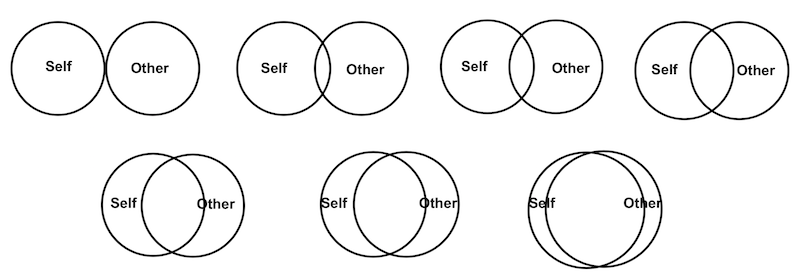
\includegraphics[width=0.8\textwidth]{assets/appendix/ios-circles.png}
\caption{The Inclusion of Other in the Self (IOS) Scale showing seven options with increasing degrees of overlap between "Self" and "Other" circles. Adapted from \cite{aron1991close}.}
\label{fig:ios-scale}
\end{figure}

Participants selected from Option 1 (no overlap) to Option 7 (almost complete overlap) to indicate their perceived closeness with their partner. The scale provides a quick, intuitive measure of interpersonal closeness that has been validated across numerous relationship contexts \cite{aron1991close}.

\subsection{Perceived Competence Scale (PCS)}
\label{appendix:pcs}

Participants rated each statement on a 7-point Likert scale: \textbf{Not at all true} - \textbf{Slightly true} - \textbf{Somewhat true} - \textbf{Moderately true} - \textbf{Fairly true} - \textbf{Very true} - \textbf{Extremely true}. This questionnaire was administered twice: once before the study and once after. Participants completed both self-assessment and partner assessment versions.

\subsubsection{Self-Assessment Items}
\begin{enumerate}
    \item I feel confident in my ability to collaborate and perform well in the task with my partner.
    \item I am capable of collaborating and performing well in the task with my partner.
    \item I am able to collaborate and perform well with my partner.
    \item I feel able to meet the challenge of collaborating and performing well in the task with my partner.
\end{enumerate}

\subsubsection{Partner Assessment Items}
\begin{enumerate}
    \item I feel confident in my partner's ability to collaborate and perform well in the task with me.
    \item My partner is capable of collaborating and performing well in the task with me.
    \item My partner is able to collaborate and perform well with me.
    \item My partner is able to meet the challenge of collaborating and performing well in the task with me.
\end{enumerate}

\subsection{Dyadic Trust Scale (DTS)}
\label{appendix:dts}

Participants rated each statement on a 7-point Likert scale: \textbf{Not at all true} - \textbf{Slightly true} - \textbf{Somewhat true} - \textbf{Moderately true} - \textbf{Fairly true} - \textbf{Very true} - \textbf{Extremely true}. This questionnaire was administered twice: once before the study and once after.

\begin{enumerate}
    \item My partner is primarily interested in his (her) own welfare.
    \item There are times when my partner cannot be trusted.
    \item My partner is perfectly honest and truthful with me.
    \item I feel that I can trust my partner completely.
    \item My partner is truly sincere in his (her) promises.
    \item I feel that my partner does not show me enough consideration.
    \item My partner treats me fairly and justly.
    \item I feel that my partner can be counted on to help me.
\end{enumerate}

\section{Interview and Discussion Protocols}

\subsection{Individual Semi-Structured Interview Protocol}
\label{appendix:individual-interview}

The following protocol was used for individual semi-structured interviews conducted after completion of all four task variants. Each interview lasted approximately 10-15 minutes.

\subsubsection{General Experience}
\begin{itemize}
    \item Can you briefly share your overall experience with the task today?
    \item Were there moments you particularly enjoyed or felt frustrated? Can you describe them?
    \item Was there a particular task variant that stood out? Why?
\end{itemize}

\subsubsection{Task Performance}
\begin{itemize}
    \item How do you feel about your performance?
    \item How about your partner's performance?
\end{itemize}

\subsubsection{Collaboration}
\begin{itemize}
    \item How would you describe your communication style with your partner during the tasks?
    \item Did it differ between variants?
\end{itemize}

\subsubsection{Personality}
\begin{itemize}
    \item Did you feel your personality or previous experience played a role in how you collaborated?
    \item How well did you and your partner communicate and adapt to each other's working styles?
\end{itemize}

\subsubsection{Cognitive Load}
\begin{itemize}
    \item Did you feel mentally overloaded at any point? If so, when?
    \item How would you compare the difficulty of the task across the different conditions?
\end{itemize}

\subsection{Joint Semi-Structured Discussion Protocol}
\label{appendix:joint-discussion}

The following protocol was used for joint semi-structured discussions conducted after both individual interviews were completed. Each discussion lasted approximately 5 minutes.

\subsubsection{Warm-up}
\begin{itemize}
    \item "So, overall---how was that for you two? Anything surprising or memorable?"
\end{itemize}

\subsubsection{Collaboration \& Communication}
\begin{itemize}
    \item "Did you feel you were on the same page during the building task?"
    \item "Was there a moment when you really clicked, or when you had trouble getting through to each other?"
\end{itemize}

\subsubsection{Problem-Solving Style}
\begin{itemize}
    \item Who contributed/took initiative more during different phases of the task?
    \item How were responsibilities distributed between you?
\end{itemize}

\subsubsection{Wrap-Up Thoughts}
\begin{itemize}
    \item "If you were going to build another bridge together tomorrow, what's one thing you'd want to do differently?"
\end{itemize} 